% !TEX root = ../main.tex
\chapter{Introduction}
\label{chapter:Introduction}


\begin{itemize}
	\item Set scene. What problem are we solving and why?
	\item Describe different approaches
	\item Describe new insight
	\item Describe remainder of paper
\end{itemize}


	This document has been created in order to show you some of the capabilities of \LaTeX.  A great resource for an introduction to \LaTeX\xspace is Tobias
Oetiker's ''The Not So Short Introduction to \LaTeXe'' \cite{latex}.  Please
page through that document
before starting with your thesis.
\par
Anyways your introduction goes here.


Below a few \LaTeX examples are included for beginners
\comment{You can also put comments in the margins for you or your advisor}
\begin{figure}[ht]
  \centering
  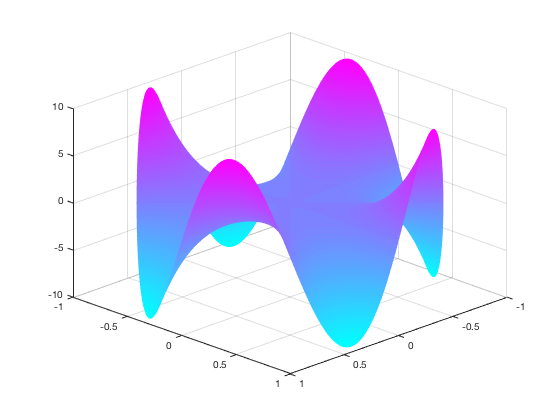
\includegraphics[width=5cm]{images/swing_function_plot.png}
  \caption{$u(x)$}%{Numerically solved solution}
  \label{fig:swingPlot}
\end{figure}


Equations can also be labeled
\begin{equation}
	\pi = \mathrm{e}^{i\cdot\phi}
	\label{eq:equation1}
\end{equation}


And later referenced. Even in subfigures.
\begin{figure}[!htb]
  \centering
  \begin{subfigure}[b]{0.3\textwidth}
    \centering
  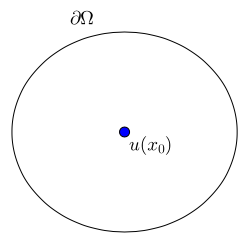
\includegraphics[width=\textwidth]{images/CircCenter}
  \caption{Equation \ref{eq:equation1}}\label{fig:circcenter}
\end{subfigure}
\hfill
  \begin{subfigure}[b]{0.3\textwidth}
    \centering
  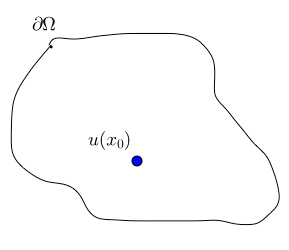
\includegraphics[width=\textwidth]{images/GeneralOffset}
  \label{fig:generaloffset}
  \caption{Equation \ref{eq:equation1}}
\end{subfigure}
\end{figure}
\section{Including code}

Code can be using the package
\href{https://www.sharelatex.com/learn/Code\_Highlighting\_with\_minted}{Minted}.

An exaple of which of can be found below (see Source Code \ref{lst:nice_listing})
\begin{listing}
	%the language syntax can be declared here.
	\begin{minted}{python} 
	import numpy as np
	\end{minted}

  \caption{My nice listing}
  \label{lst:nice_listing}
\end{listing}
